\documentclass[10pt,a4paper]{report}
\usepackage{geometry}
\usepackage{fontspec}
\usepackage{hyperref}
\usepackage{graphicx}
\usepackage{booktabs}
\usepackage{tabularx}
\usepackage{longtable}
\usepackage{array}
\usepackage{enumitem}
\setlist{topsep=2pt, itemsep=1pt, parsep=1pt, partopsep=0pt}
\usepackage{xcolor}
\usepackage{titlesec}
\usepackage{fancyhdr}
\usepackage{amsmath}
\usepackage{amssymb}
\usepackage{tikz}
\usetikzlibrary{positioning, shapes.geometric, arrows.meta, calc, shadows, backgrounds, fit, decorations.pathreplacing, shapes.multipart, mindmap, trees}
\usepackage{float}
\setlength{\textfloatsep}{8pt}
\setlength{\floatsep}{6pt}
\setlength{\intextsep}{6pt}
\usepackage{listings}
\usepackage{caption}
\usepackage{subcaption}
\usepackage{tcolorbox}
\tcbuselibrary{skins, breakable, listings}
\usepackage{pgfplots}
\pgfplotsset{compat=1.18}
\usepackage{algorithm}
\usepackage{algpseudocode}
\usepackage{multicol}
\usepackage{wrapfig}
\usepackage{soul}
\usepackage{pifont}
\usepackage{textcomp}

%------------------------------------------------------------------------------
% Fonts and layout (XeLaTeX)
%------------------------------------------------------------------------------
\setmainfont{Latin Modern Roman}
\setsansfont{Latin Modern Sans}
\setmonofont{Latin Modern Mono}
\geometry{margin=0.65in, headheight=14pt, top=0.6in, bottom=0.55in}
\usepackage{setspace}
\setstretch{0.95}

% Color palette - Professional academic theme
\definecolor{tmBlue}{RGB}{6,101,160}
\definecolor{tmDarkBlue}{RGB}{4,70,115}
\definecolor{tmLight}{RGB}{226,243,255}
\definecolor{tmLighter}{RGB}{245,250,255}
\definecolor{tmGray}{RGB}{73,85,104}
\definecolor{tmDarkGray}{RGB}{45,52,65}
\definecolor{tmAccent}{RGB}{240,113,36}
\definecolor{tmGreen}{RGB}{46,139,87}
\definecolor{tmRed}{RGB}{178,34,34}
\definecolor{tmGold}{RGB}{218,165,32}
\definecolor{tmPurple}{RGB}{128,0,128}

% Custom checkmark and crossmark
\newcommand{\cmark}{\textcolor{tmGreen}{\ding{51}}}
\newcommand{\xmark}{\textcolor{tmRed}{\ding{55}}}

% Hyperref setup
\hypersetup{
	colorlinks=true,
	linkcolor=tmBlue,
	urlcolor=tmAccent,
	citecolor=tmBlue,
	pdftitle={TuniMaqam API - Technical Report},
	pdfauthor={TuniMaqam Engineering Team},
	pdfsubject={Pedagogical Maqam Intelligence Platform}
}

% Heading tweaks with decorative elements
\titleformat{\chapter}[display]
{\bfseries\Large\color{tmBlue}}
{\filright\MakeUppercase{\chaptertitlename}\ \Large\thechapter}
{0.5ex}
{\titlerule[1.5pt]\vspace{0.5ex}}
[\vspace{0.5ex}\titlerule]

\titleformat{\section}{\bfseries\large\color{tmBlue}}{\thesection}{6pt}{}[\vspace{1pt}\color{tmLight}\hrule height 0.5pt]
\titleformat{\subsection}{\bfseries\normalsize\color{tmDarkBlue}}{\thesubsection}{5pt}{}
\titleformat{\subsubsection}{\bfseries\small\color{tmGray}}{\thesubsubsection}{4pt}{}

\titlespacing*{\chapter}{0pt}{12pt}{10pt}
\titlespacing*{\section}{0pt}{8pt}{4pt}
\titlespacing*{\subsection}{0pt}{6pt}{3pt}
\titlespacing*{\subsubsection}{0pt}{4pt}{2pt}

% Header/Footer with decorative line
\pagestyle{fancy}
\fancyhf{}
\fancyhead[L]{\textcolor{tmGray}{\small\leftmark}}
\fancyhead[R]{\textcolor{tmBlue}{\small TuniMaqam API}}
\fancyfoot[C]{\textcolor{tmGray}{\thepage}}
\renewcommand{\headrulewidth}{0.4pt}
\renewcommand{\footrulewidth}{0.2pt}
\renewcommand{\headrule}{\hbox to\headwidth{\color{tmBlue}\leaders\hrule height \headrulewidth\hfill}}

% Custom tcolorbox styles
\newtcolorbox{infobox}[1][]{
	enhanced,
	colback=tmLight,
	colframe=tmBlue,
	fonttitle=\bfseries,
	boxrule=0.5pt,
	arc=2mm,
	left=4pt, right=4pt, top=4pt, bottom=4pt,
	#1
}

\newtcolorbox{warningbox}[1][]{
	enhanced,
	colback=yellow!10,
	colframe=tmAccent,
	fonttitle=\bfseries,
	boxrule=0.5pt,
	arc=2mm,
	left=4pt, right=4pt,
	#1
}

\newtcolorbox{successbox}[1][]{
	enhanced,
	colback=green!5,
	colframe=tmGreen,
	fonttitle=\bfseries,
	boxrule=0.5pt,
	arc=2mm,
	left=4pt, right=4pt,
	#1
}

\newtcolorbox{keyconceptbox}[2][]{
	enhanced,
	colback=tmLighter,
	colframe=tmDarkBlue,
	fonttitle=\bfseries\color{white},
	colbacktitle=tmDarkBlue,
	coltitle=white,
	title=#2,
	boxrule=1pt,
	arc=3mm,
	left=6pt, right=6pt, top=4pt, bottom=4pt,
	attach boxed title to top left={xshift=5mm,yshift=-2mm},
	boxed title style={arc=2mm, boxrule=0pt},
	#1
}

% Listings for JSON / code snippets - Enhanced
\lstdefinestyle{tmjson}{
	basicstyle=\ttfamily\small,
	backgroundcolor=\color{tmLighter},
	frame=single,
	rulecolor=\color{tmBlue},
	breaklines=true,
	keywordstyle=\color{tmBlue}\bfseries,
	stringstyle=\color{tmAccent},
	commentstyle=\color{tmGray}\itshape,
	numbers=left,
	numberstyle=\tiny\color{tmGray},
	numbersep=8pt,
	xleftmargin=15pt,
	showstringspaces=false
}

\lstdefinestyle{tmpython}{
	language=Python,
	basicstyle=\ttfamily\small,
	backgroundcolor=\color{tmLighter},
	frame=single,
	rulecolor=\color{tmBlue},
	breaklines=true,
	keywordstyle=\color{tmBlue}\bfseries,
	stringstyle=\color{tmGreen},
	commentstyle=\color{tmGray}\itshape,
	numbers=left,
	numberstyle=\tiny\color{tmGray},
	numbersep=8pt,
	xleftmargin=15pt,
	showstringspaces=false,
	morekeywords={def,class,return,import,from,as,if,else,elif,for,while,try,except,with,True,False,None}
}

% Convenience table column
\newcolumntype{Y}{>{\raggedright\arraybackslash}X}
\newcolumntype{C}[1]{>{\centering\arraybackslash}p{#1}}
\newcolumntype{L}[1]{>{\raggedright\arraybackslash}p{#1}}
\newcolumntype{R}[1]{>{\raggedleft\arraybackslash}p{#1}}

% Custom commands for emphasis
\newcommand{\tech}[1]{\texttt{\textcolor{tmBlue}{#1}}}
\newcommand{\api}[1]{\texttt{\textcolor{tmGreen}{#1}}}
\newcommand{\important}[1]{\textbf{\textcolor{tmAccent}{#1}}}

\setlength{\parskip}{3pt plus 1pt minus 1pt}
\setlength{\parindent}{0.8em}

\begin{document}

%------------------------------------------------------------------------------
% Title Page
%------------------------------------------------------------------------------
\begin{titlepage}
\newgeometry{margin=1in}
\centering

\vspace*{1cm}

% Institution
{\Large\textsc{Tunis Business School}\\[0.3cm]}
{\large\textsc{Information Technology -- Business Analytics}\\[0.2cm]}

\vspace{2cm}

% Decorative line
{\color{tmBlue}\rule{0.5\textwidth}{1pt}}

\vspace{1.2cm}

% Main title
{\fontsize{38}{44}\selectfont\bfseries\color{tmBlue} TuniMaqam API\\[1cm]}
{\Large A REST API Platform for Tunisian Maqam heritage (\textit{Ṭbu'a})\\[0.4cm]}
{\large Preservation, Education, and Discovery}

\vspace{1.2cm}

% Decorative line
{\color{tmBlue}\rule{0.5\textwidth}{1pt}}

\vspace{2.5cm}

% Info table
\begin{tabular}{@{}r@{\hspace{0.8cm}}l@{}}
\textbf{Author} & Roua Smida \\[0.4cm]
\textbf{Specialization} & IT--BA \\[0.4cm]
\textbf{Course} & IT325 Web Services \\[0.4cm]
\textbf{Supervisor} & Dr. Montassar Ben Messaoud \\[0.4cm]
\textbf{Academic Year} & 2025--2026 \\
\end{tabular}

\vfill

\restoregeometry
\end{titlepage}

\pagenumbering{roman}

%------------------------------------------------------------------------------
% Abstract
%------------------------------------------------------------------------------
\chapter*{Abstract}
\addcontentsline{toc}{chapter}{Abstract}

Tunisian maqam music represents a rich cultural heritage that faces the threat of gradual erosion in the modern era. This project presents \textbf{TuniMaqam}, a comprehensive REST API platform designed to preserve, educate, and promote Tunisian maqamet through intelligent technology.

The system implements four core services: (1) a \textbf{Knowledge Service} providing a structured repository of maqam metadata with community-driven contributions; (2) a \textbf{Learning Service} offering adaptive, gamified educational experiences including quizzes, flashcards, and interactive exercises; (3) an \textbf{Analysis Engine} employing mathematical confidence scoring algorithms for maqam identification from note sequences and audio inputs; and (4) a \textbf{Recommendation Engine} utilizing multi-factor contextual scoring for culturally-appropriate maqam suggestions.

The platform is built using Flask with SQLAlchemy ORM, secured through JWT authentication with role-based access control, and integrates AssemblyAI for audio transcription. Testing validates all core functionalities, and the system is containerized for scalable deployment.

\textbf{Keywords:} Maqam, Tunisian Music, REST API, Cultural Preservation, E-Learning, Flask, Python

\newpage

\tableofcontents
\newpage
\pagenumbering{arabic}

%------------------------------------------------------------------------------
\chapter{General Introduction}
%------------------------------------------------------------------------------

\section{Context and Motivation}

Tunisia's maqam tradition---known locally as \textit{ṭab'} (singular) or \textit{ṭbūʿ} (plural)---represents one of the Arab world's most sophisticated and emotionally rich musical systems. This living heritage has accompanied weddings, mourning, celebrations, and spiritual gatherings for centuries. Unlike Western music's major/minor dichotomy, the maqam system encompasses dozens of distinct modal frameworks, each carrying specific emotional connotations and cultural contexts.

Yet, like many oral traditions, this heritage faces the relentless erosion of time. Master musicians pass away without transferring their complete knowledge; younger generations gravitate toward globalized musical forms; and the subtle nuances distinguishing one ṭab' from another risk being forgotten.

\section{Problem Statement}

\begin{keyconceptbox}{The Challenge}
How can we leverage modern technology to preserve, teach, and promote Tunisian maqam music while respecting its cultural authenticity and making it accessible to a global audience?
\end{keyconceptbox}

Current challenges include:
\begin{itemize}[leftmargin=0.6cm, topsep=4pt, itemsep=2pt]
	\item \textbf{Fragmented Knowledge:} Maqam information exists in scattered, often inaccessible sources
	\item \textbf{Learning Barriers:} Traditional maqam education requires years of apprenticeship
	\item \textbf{Identification Difficulty:} Even experienced musicians struggle to identify rare maqamet
	\item \textbf{Cultural Context Loss:} Understanding which maqam suits which occasion requires deep cultural knowledge
\end{itemize}

\section{Proposed Solution}

\textbf{TuniMaqam} is a comprehensive Flask-based REST API that curates Tunisian maqamet, powers adaptive learning experiences, and delivers culturally-sensitive recommendations. The platform combines structured musical knowledge, gamified learning tools, and intelligent audio/note analysis to guide learners from beginners to accomplished practitioners.

\section{Project Objectives}

\begin{enumerate}[leftmargin=0.8cm, topsep=4pt, itemsep=2pt]
	\item \textbf{Preservation:} Create a structured, extensible database of Tunisian maqamet with community contribution capabilities
	\item \textbf{Education:} Develop adaptive learning tools that make maqam education accessible and engaging
	\item \textbf{Analysis:} Implement intelligent algorithms for maqam identification from musical input
	\item \textbf{Recommendation:} Build context-aware systems that suggest appropriate maqamet for occasions
	\item \textbf{Accessibility:} Provide a secure, documented API for integration with various applications
\end{enumerate}

\section{Mission}

TuniMaqam's mission: \textbf{Preserve} Tunisian maqamet (especially rare forms), \textbf{Educate} through accessible and engaging learning, and \textbf{Connect} generations with the global music community.

\section{Related Work}

Existing solutions in cultural heritage digitization (Europeana, Arab Music Archiving) focus on passive archival without interactive learning. Music education platforms (Yousician, Teoria) provide gamified learning but none address maqam systems. Academic research in maqam recognition \cite{gedik2010, salamon2012} focuses on pitch analysis but lacks integrated educational tools. \textbf{Research Gap:} No existing system combines structured Tunisian maqam knowledge, adaptive learning, intelligent analysis, and contextual recommendations in an accessible API format. TuniMaqam addresses this gap.

\section{System Class Diagram}

\begin{figure}[H]
	\centering
	\includegraphics[width=\textwidth]{TuniMaqam Class Diagram.png}
	\caption{TuniMaqam Class Diagram}
	\label{fig:classdiagram}
\end{figure}

%------------------------------------------------------------------------------
\chapter{Requirements Analysis}
%------------------------------------------------------------------------------

This chapter presents the functional and non-functional requirements derived from stakeholder analysis and domain research.

\section{Stakeholder Analysis}

\begin{center}
\begin{tabular}{p{0.20\textwidth}p{0.35\textwidth}p{0.35\textwidth}}
\toprule
\textbf{Stakeholder} & \textbf{Role} & \textbf{Needs}\\
\midrule
Learners & Primary users & Easy learning, progress tracking\\
Musicians & Content contributors & Share knowledge, gain recognition\\
Researchers & Data consumers & Access structured maqam data\\
Developers & API integrators & Clear documentation, stable API\\
Administrators & System managers & User management, content moderation\\
\bottomrule
\end{tabular}
\end{center}

\section{Functional Requirements}

\begin{longtable}{p{0.08\textwidth}p{0.25\textwidth}p{0.52\textwidth}p{0.08\textwidth}}
\toprule
\textbf{ID} & \textbf{Requirement} & \textbf{Description} & \textbf{Priority}\\
\midrule
\endhead
FR-01 & Maqam Retrieval & System shall allow users to retrieve maqam information by ID, name, or region & High\\
FR-02 & Maqam Creation & Admins shall be able to create new maqam entries with full metadata & High\\
FR-03 & Contribution Submission & Users shall submit contributions for review & High\\
FR-04 & Contribution Review & Experts/admins shall approve or reject contributions & High\\
FR-05 & Quiz Generation & System shall generate adaptive quizzes based on user level & High\\
FR-06 & Quiz Scoring & System shall score answers and provide explanations & High\\
FR-07 & Flashcard Generation & System shall generate flashcards by topic & Medium\\
FR-08 & Matching Exercises & System shall provide maqam-attribute matching exercises & Medium\\
FR-09 & Ordering Exercises & System shall provide jins ordering exercises & Medium\\
FR-10 & Note Analysis & System shall identify maqam candidates from note input & High\\
FR-11 & Audio Analysis & System shall extract notes from audio and identify maqamet & Medium\\
FR-12 & Recommendations & System shall recommend maqamet based on context & High\\
FR-13 & User Authentication & System shall authenticate users via JWT and Google OAuth & High\\
FR-14 & Role Management & System shall enforce role-based access control & High\\
FR-15 & Activity Logging & System shall log all user learning activities & Medium\\
\bottomrule
\end{longtable}

\section{Non-Functional Requirements}

\begin{longtable}{p{0.10\textwidth}p{0.20\textwidth}p{0.55\textwidth}p{0.08\textwidth}}
\toprule
\textbf{ID} & \textbf{Category} & \textbf{Requirement} & \textbf{Priority}\\
\midrule
\endhead
NFR-01 & Performance & API responses shall complete within 500ms for 95\% of requests & High\\
NFR-02 & Scalability & System shall support horizontal scaling via containerization & Medium\\
NFR-03 & Security & All endpoints shall be protected against OWASP Top 10 vulnerabilities & High\\
NFR-04 & Availability & System shall maintain 99\% uptime during operating hours & High\\
NFR-05 & Usability & API shall follow RESTful conventions with Swagger documentation & High\\
NFR-06 & Maintainability & Code shall follow PEP 8 standards with >80\% test coverage & Medium\\
NFR-07 & Portability & System shall run on any Docker-compatible platform & Medium\\
NFR-08 & Localization & System shall support bilingual content (Arabic/English) & Medium\\
\bottomrule
\end{longtable}

\section{Use Case Diagram}

\begin{figure}[H]
\centering
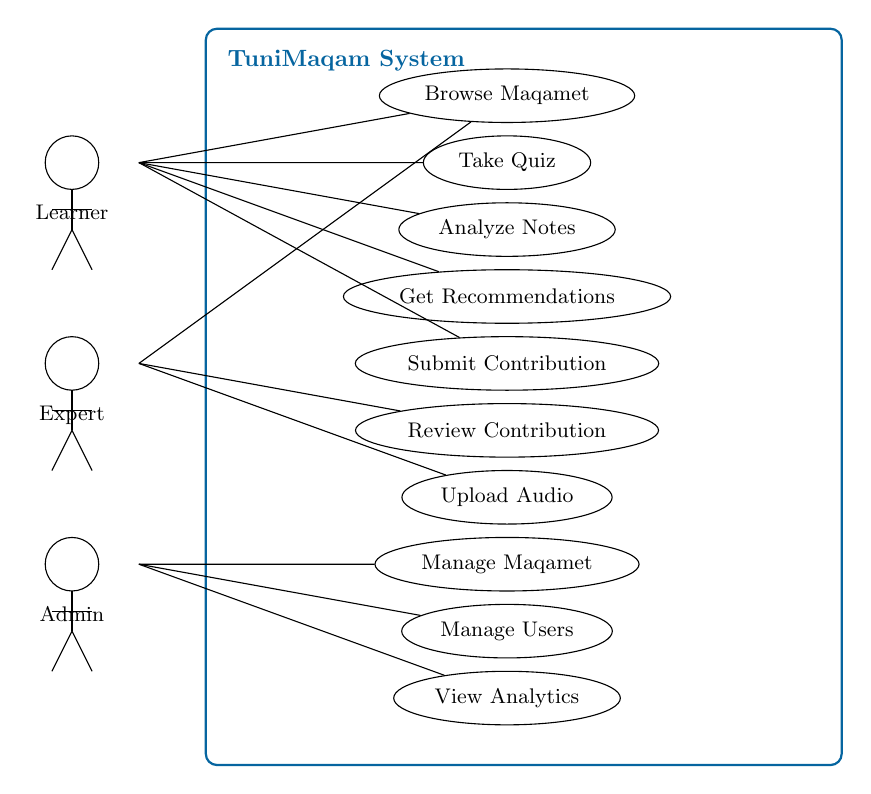
\begin{tikzpicture}[scale=0.85, transform shape]
	% System boundary
	\draw[thick, rounded corners, tmBlue] (-0.5,-6) rectangle (9,5);
	\node[anchor=north west, tmBlue, font=\bfseries] at (-0.3,4.8) {TuniMaqam System};
	
	% Actors
	\node[circle, draw, minimum size=0.8cm] (learner) at (-2.5,3) {};
	\node[below=0.1cm of learner, font=\small] {Learner};
	\draw (-2.5,2.6) -- (-2.5,2);
	\draw (-2.8,2.3) -- (-2.2,2.3);
	\draw (-2.5,2) -- (-2.8,1.4);
	\draw (-2.5,2) -- (-2.2,1.4);
	
	\node[circle, draw, minimum size=0.8cm] (expert) at (-2.5,0) {};
	\node[below=0.1cm of expert, font=\small] {Expert};
	\draw (-2.5,-0.4) -- (-2.5,-1);
	\draw (-2.8,-0.7) -- (-2.2,-0.7);
	\draw (-2.5,-1) -- (-2.8,-1.6);
	\draw (-2.5,-1) -- (-2.2,-1.6);
	
	\node[circle, draw, minimum size=0.8cm] (admin) at (-2.5,-3) {};
	\node[below=0.1cm of admin, font=\small] {Admin};
	\draw (-2.5,-3.4) -- (-2.5,-4);
	\draw (-2.8,-3.7) -- (-2.2,-3.7);
	\draw (-2.5,-4) -- (-2.8,-4.6);
	\draw (-2.5,-4) -- (-2.2,-4.6);
	
	% Use cases
	\node[ellipse, draw, minimum width=2.5cm, minimum height=0.8cm, align=center, font=\small] (uc1) at (4,4) {Browse Maqamet};
	\node[ellipse, draw, minimum width=2.5cm, minimum height=0.8cm, align=center, font=\small] (uc2) at (4,3) {Take Quiz};
	\node[ellipse, draw, minimum width=2.5cm, minimum height=0.8cm, align=center, font=\small] (uc3) at (4,2) {Analyze Notes};
	\node[ellipse, draw, minimum width=2.5cm, minimum height=0.8cm, align=center, font=\small] (uc4) at (4,1) {Get Recommendations};
	\node[ellipse, draw, minimum width=2.5cm, minimum height=0.8cm, align=center, font=\small] (uc5) at (4,0) {Submit Contribution};
	\node[ellipse, draw, minimum width=2.5cm, minimum height=0.8cm, align=center, font=\small] (uc6) at (4,-1) {Review Contribution};
	\node[ellipse, draw, minimum width=2.5cm, minimum height=0.8cm, align=center, font=\small] (uc7) at (4,-2) {Upload Audio};
	\node[ellipse, draw, minimum width=2.5cm, minimum height=0.8cm, align=center, font=\small] (uc8) at (4,-3) {Manage Maqamet};
	\node[ellipse, draw, minimum width=2.5cm, minimum height=0.8cm, align=center, font=\small] (uc9) at (4,-4) {Manage Users};
	\node[ellipse, draw, minimum width=2.8cm, minimum height=0.8cm, align=center, font=\small] (uc10) at (4,-5) {View Analytics};
	
	% Connections
	\draw (-1.5,3) -- (uc1);
	\draw (-1.5,3) -- (uc2);
	\draw (-1.5,3) -- (uc3);
	\draw (-1.5,3) -- (uc4);
	\draw (-1.5,3) -- (uc5);
	
	\draw (-1.5,0) -- (uc1);
	\draw (-1.5,0) -- (uc6);
	\draw (-1.5,0) -- (uc7);
	
	\draw (-1.5,-3) -- (uc8);
	\draw (-1.5,-3) -- (uc9);
	\draw (-1.5,-3) -- (uc10);
\end{tikzpicture}
\caption{Use Case Diagram showing actor interactions with TuniMaqam}
\label{fig:usecase}
\end{figure}

%------------------------------------------------------------------------------
\chapter{System Design and Architecture}
%------------------------------------------------------------------------------

This chapter presents the architectural design decisions and UML models for TuniMaqam.

\section{Architectural Pattern}

TuniMaqam follows a \textbf{layered architecture} with clear separation of concerns:

\begin{figure}[H]
\centering
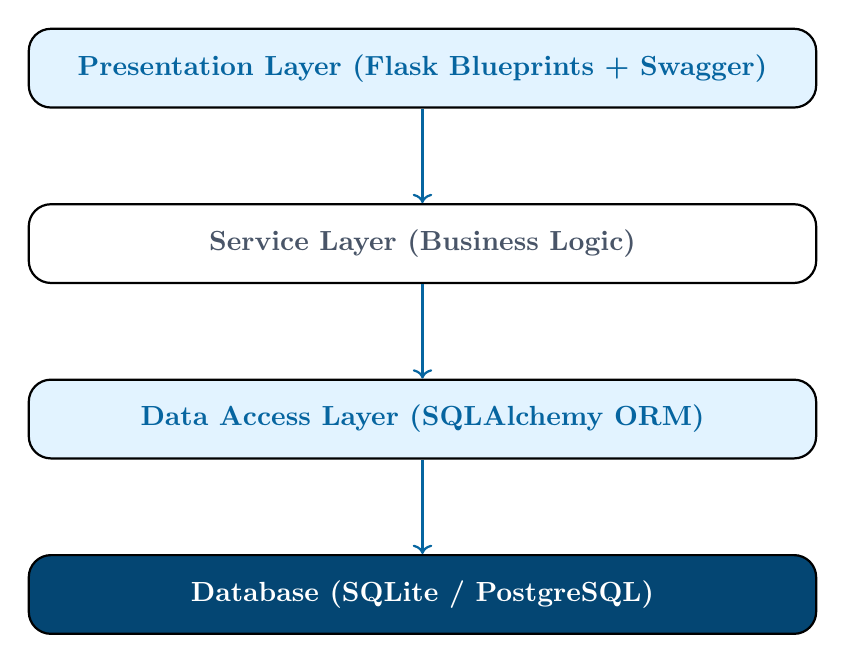
\begin{tikzpicture}[node distance=1.2cm]
	\node[draw, thick, rounded corners=8pt, minimum width=10cm, minimum height=1cm, fill=tmLight, text=tmBlue, font=\bfseries] (presentation) {Presentation Layer (Flask Blueprints + Swagger)};
	\node[draw, thick, rounded corners=8pt, below=of presentation, minimum width=10cm, minimum height=1cm, fill=white, text=tmGray, font=\bfseries] (service) {Service Layer (Business Logic)};
	\node[draw, thick, rounded corners=8pt, below=of service, minimum width=10cm, minimum height=1cm, fill=tmLight, text=tmBlue, font=\bfseries] (data) {Data Access Layer (SQLAlchemy ORM)};
	\node[draw, thick, rounded corners=8pt, below=of data, minimum width=10cm, minimum height=1cm, fill=tmDarkBlue, text=white, font=\bfseries] (db) {Database (SQLite / PostgreSQL)};
	\draw[->, thick, tmBlue] (presentation) -- (service);
	\draw[->, thick, tmBlue] (service) -- (data);
	\draw[->, thick, tmBlue] (data) -- (db);
\end{tikzpicture}
\caption{Layered Architecture of TuniMaqam}
\label{fig:layers}
\end{figure}

\section{Component Diagram}

\begin{figure}[H]
\centering
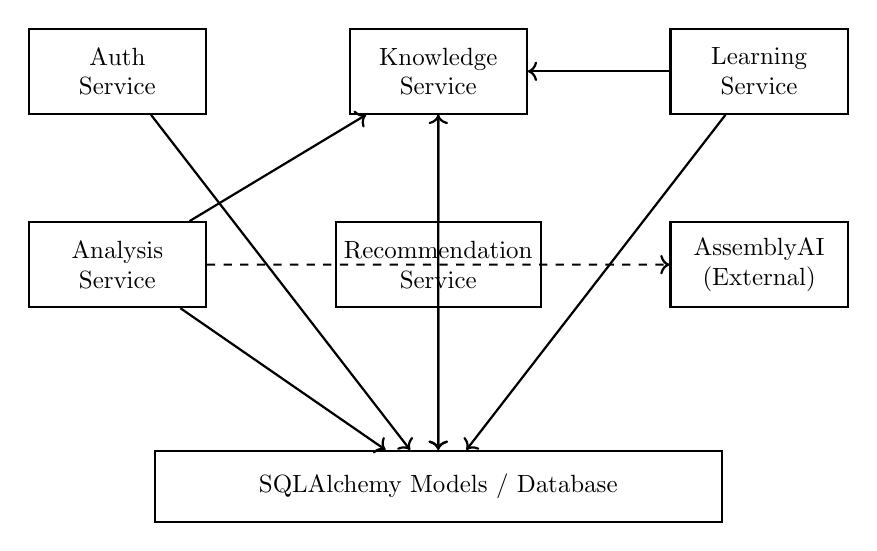
\begin{tikzpicture}[node distance=1.5cm and 2cm, scale=0.9, transform shape]
	% Components
	\node[draw, thick, minimum width=2.5cm, minimum height=1.2cm, align=center] (auth) {Auth\\Service};
	\node[draw, thick, minimum width=2.5cm, minimum height=1.2cm, align=center, right=of auth] (knowledge) {Knowledge\\Service};
	\node[draw, thick, minimum width=2.5cm, minimum height=1.2cm, align=center, right=of knowledge] (learning) {Learning\\Service};
	\node[draw, thick, minimum width=2.5cm, minimum height=1.2cm, align=center, below=of auth] (analysis) {Analysis\\Service};
	\node[draw, thick, minimum width=2.5cm, minimum height=1.2cm, align=center, below=of knowledge] (recommend) {Recommendation\\Service};
	\node[draw, thick, minimum width=2.5cm, minimum height=1.2cm, align=center, below=of learning] (external) {AssemblyAI\\(External)};
	\node[draw, thick, minimum width=8cm, minimum height=1cm, align=center, below=2cm of recommend] (db) {SQLAlchemy Models / Database};
	
	% Connections
	\draw[->, thick] (auth) -- (db);
	\draw[->, thick] (knowledge) -- (db);
	\draw[->, thick] (learning) -- (db);
	\draw[->, thick] (analysis) -- (db);
	\draw[->, thick] (recommend) -- (db);
	\draw[->, thick] (analysis) -- (knowledge);
	\draw[->, thick] (recommend) -- (knowledge);
	\draw[->, thick] (learning) -- (knowledge);
	\draw[->, thick, dashed] (analysis) -- (external);
\end{tikzpicture}
\caption{Component Diagram showing service interactions}
\label{fig:component}
\end{figure}

\section{Entity-Relationship Diagram}

\begin{figure}[H]
\centering
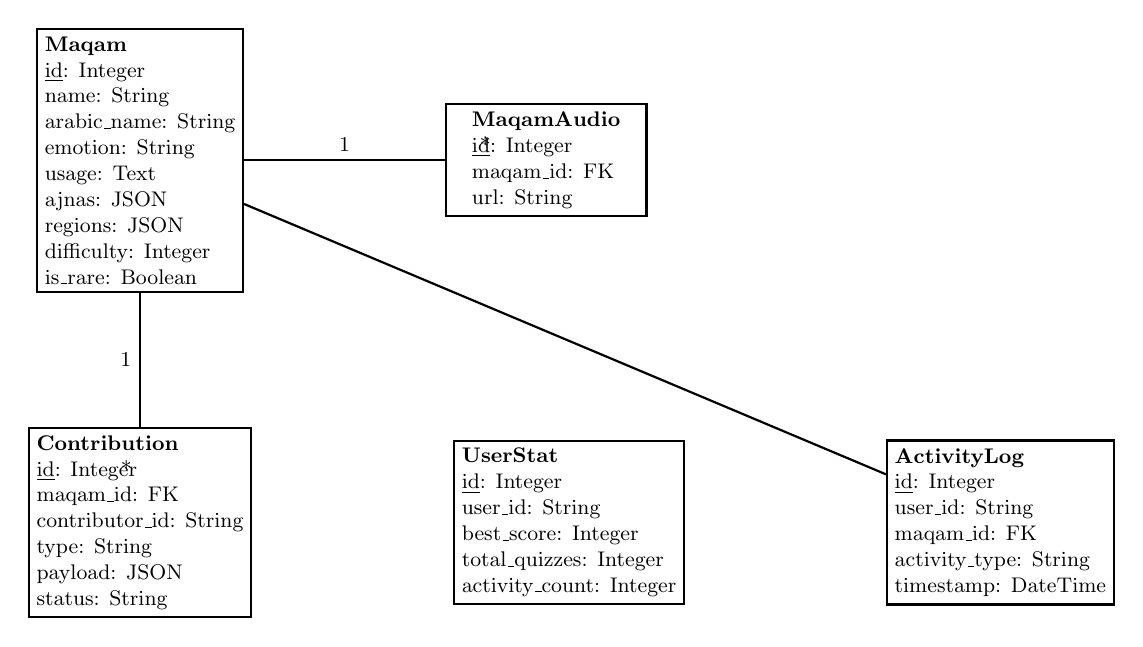
\begin{tikzpicture}[node distance=2cm and 3cm, scale=0.85, transform shape]
	% Entities
	\node[draw, thick, rectangle, minimum width=3cm, minimum height=2.5cm, align=left, font=\small] (maqam) {
		\textbf{Maqam}\\
		\underline{id}: Integer\\
		name: String\\
		arabic\_name: String\\
		emotion: String\\
		usage: Text\\
		ajnas: JSON\\
		regions: JSON\\
		difficulty: Integer\\
		is\_rare: Boolean
	};
	
	\node[draw, thick, rectangle, minimum width=3cm, minimum height=1.5cm, align=left, font=\small, right=of maqam] (audio) {
		\textbf{MaqamAudio}\\
		\underline{id}: Integer\\
		maqam\_id: FK\\
		url: String
	};
	
	\node[draw, thick, rectangle, minimum width=3cm, minimum height=2cm, align=left, font=\small, below=of maqam] (contrib) {
		\textbf{Contribution}\\
		\underline{id}: Integer\\
		maqam\_id: FK\\
		contributor\_id: String\\
		type: String\\
		payload: JSON\\
		status: String
	};
	
	\node[draw, thick, rectangle, minimum width=3cm, minimum height=1.8cm, align=left, font=\small, right=of contrib] (userstat) {
		\textbf{UserStat}\\
		\underline{id}: Integer\\
		user\_id: String\\
		best\_score: Integer\\
		total\_quizzes: Integer\\
		activity\_count: Integer
	};
	
	\node[draw, thick, rectangle, minimum width=3cm, minimum height=1.5cm, align=left, font=\small, right=of userstat] (activity) {
		\textbf{ActivityLog}\\
		\underline{id}: Integer\\
		user\_id: String\\
		maqam\_id: FK\\
		activity\_type: String\\
		timestamp: DateTime
	};
	
	% Relationships
	\draw[thick] (maqam) -- node[above, font=\small] {1} (audio);
	\node[font=\small] at ($(maqam)!0.85!(audio)$) [above] {*};
	
	\draw[thick] (maqam) -- node[left, font=\small] {1} (contrib);
	\node[font=\small] at ($(maqam)!0.85!(contrib)$) [left] {*};
	
	\draw[thick] (maqam) -- (activity);
\end{tikzpicture}
\caption{Entity-Relationship Diagram for TuniMaqam data model}
\label{fig:erd}
\end{figure}

\section{Sequence Diagram: Quiz Flow}

\begin{figure}[H]
\centering
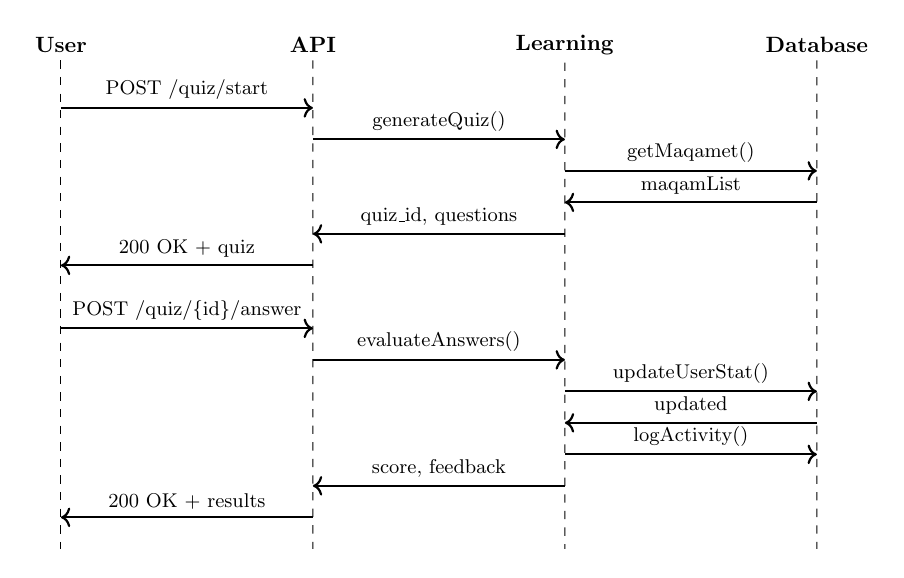
\begin{tikzpicture}[scale=0.8, transform shape]
	% Lifelines
	\node (user) at (0,0) {\textbf{User}};
	\node (api) at (4,0) {\textbf{API}};
	\node (learning) at (8,0) {\textbf{Learning}};
	\node (db) at (12,0) {\textbf{Database}};
	
	\draw[dashed] (user) -- (0,-8);
	\draw[dashed] (api) -- (4,-8);
	\draw[dashed] (learning) -- (8,-8);
	\draw[dashed] (db) -- (12,-8);
	
	% Messages
	\draw[->, thick] (0,-1) -- node[above, font=\small] {POST /quiz/start} (4,-1);
	\draw[->, thick] (4,-1.5) -- node[above, font=\small] {generateQuiz()} (8,-1.5);
	\draw[->, thick] (8,-2) -- node[above, font=\small] {getMaqamet()} (12,-2);
	\draw[<-, thick] (8,-2.5) -- node[above, font=\small] {maqamList} (12,-2.5);
	\draw[<-, thick] (4,-3) -- node[above, font=\small] {quiz\_id, questions} (8,-3);
	\draw[<-, thick] (0,-3.5) -- node[above, font=\small] {200 OK + quiz} (4,-3.5);
	
	\draw[->, thick] (0,-4.5) -- node[above, font=\small] {POST /quiz/\{id\}/answer} (4,-4.5);
	\draw[->, thick] (4,-5) -- node[above, font=\small] {evaluateAnswers()} (8,-5);
	\draw[->, thick] (8,-5.5) -- node[above, font=\small] {updateUserStat()} (12,-5.5);
	\draw[<-, thick] (8,-6) -- node[above, font=\small] {updated} (12,-6);
	\draw[->, thick] (8,-6.5) -- node[above, font=\small] {logActivity()} (12,-6.5);
	\draw[<-, thick] (4,-7) -- node[above, font=\small] {score, feedback} (8,-7);
	\draw[<-, thick] (0,-7.5) -- node[above, font=\small] {200 OK + results} (4,-7.5);
\end{tikzpicture}
\caption{Sequence Diagram for Quiz interaction flow}
\label{fig:sequence}
\end{figure}

\section{Technology Stack}

\begin{center}
\begin{tabular}{p{0.25\textwidth}p{0.30\textwidth}p{0.35\textwidth}}
\toprule
\textbf{Category} & \textbf{Technology} & \textbf{Justification}\\
\midrule
Web Framework & Flask 3.x & Lightweight, flexible, well-documented\\
ORM & SQLAlchemy & Pythonic, database-agnostic\\
Data Validation & Marshmallow & Schema-based validation \& serialization\\
Authentication & PyJWT, Authlib & Industry-standard JWT, OAuth2\\
Documentation & Flasgger (Swagger) & Auto-generated API docs\\
Rate Limiting & Flask-Limiter & Configurable throttling\\
External API & AssemblyAI & Accurate speech-to-text\\
Database & SQLite / PostgreSQL & Development / Production\\
Containerization & Docker & Reproducible deployments\\
\bottomrule
\end{tabular}
\end{center}

\section{Data Validation with Marshmallow}

TuniMaqam employs \textbf{Marshmallow} for schema-based request validation and response serialization. This architectural choice provides several benefits:

\begin{itemize}[leftmargin=0.6cm, topsep=4pt, itemsep=2pt]
	\item \textbf{Type Safety:} Input data is validated against defined schemas before processing
	\item \textbf{Consistent Errors:} Validation failures return structured error messages with field-level details
	\item \textbf{Declarative Schemas:} Validation rules are defined once and reused across endpoints
	\item \textbf{Serialization:} Output schemas ensure consistent JSON response formatting
\end{itemize}

\subsubsection{Schema Examples}

\begin{lstlisting}[style=tmpython]
class NotesAnalysisSchema(Schema):
    notes = fields.List(fields.String(), required=True,
        validate=validate.Length(min=1, max=50))
    optional_mood = fields.String(load_default=None)

class ContributionSchema(Schema):
    type = fields.String(required=True,
        validate=validate.OneOf(["correction", "addition", "audio"]))
    payload = fields.Dict(required=True)
\end{lstlisting}

Endpoints validate input using \texttt{schema.load(data)}, which raises \texttt{ValidationError} with detailed messages if constraints are violated.

\section{Data Model}

The data model captures maqamet with their cultural essence: \textbf{Maqam} (bilingual names, emotions, usage contexts, ajnas, regions, difficulty, rarity); \textbf{MaqamAudio} (audio recordings with URLs); \textbf{MaqamContribution} (pending/accepted/rejected contributions with payload and reviewer metadata); \textbf{UserStat} (learner progress: scores, quiz counts, skill levels); \textbf{ActivityLog} (audit trail of user activities).

%------------------------------------------------------------------------------
\chapter{Core Services Implementation}
%------------------------------------------------------------------------------

This chapter details the four core services that power TuniMaqam: Knowledge, Learning, Analysis, and Recommendation.

\section{The Knowledge Service}

The Knowledge Service is the foundation of TuniMaqam---a comprehensive repository that captures the complete identity of Tunisian maqamet. It serves as the single source of truth for all maqam metadata.

\subsection{Service Architecture}

The Knowledge Service exposes RESTful endpoints for maqam discovery, contribution management, and audio asset handling:
\begin{itemize}[leftmargin=0.6cm, topsep=4pt, itemsep=2pt]
	\item \textbf{Resource Layer:} Flask blueprint \texttt{knowledge\_bp} handling HTTP requests
	\item \textbf{Data Layer:} SQLAlchemy models (Maqam, MaqamContribution, MaqamAudio)
	\item \textbf{Security Layer:} JWT-protected endpoints with role-based access control
\end{itemize}

\subsection{Core API Endpoints}

\subsubsection{Maqam Discovery}

\begin{tabularx}{\textwidth}{p{0.35\textwidth}p{0.12\textwidth}p{0.48\textwidth}}
\toprule
\textbf{Endpoint} & \textbf{Verb} & \textbf{Purpose}\\
\midrule
\texttt{/knowledge/maqam} & GET & Retrieve all maqamet; optional \texttt{?region=} filter\\
\texttt{/knowledge/maqam/\{id\}} & GET & Retrieve maqam by ID with full metadata\\
\texttt{/knowledge/maqam/by-name/\{name\}} & GET & Case-insensitive lookup by English name\\
\texttt{/knowledge/maqam/\{name\}/related} & GET & Related maqamet by emotion/region similarity\\
\texttt{/knowledge/regions} & GET & Map of regions to their associated maqamet\\
\bottomrule
\end{tabularx}

\subsubsection{Maqam Data Structure}

Each maqam record contains rich, structured metadata:

\begin{lstlisting}[style=tmjson]
{
  "id": 1,
  "name": "Rast",
  "arabic_name": "راست",
  "emotion": "joy",
  "emotion_weights": {"joy": 0.9, "spirituality": 0.5},
  "usage": "weddings, celebrations, morning performances",
  "ajnas": [
    {"name": "Rast", "notes": ["C", "D", "E half-flat", "F", "G"]},
    {"name": "Nahawand", "notes": ["G", "A", "Bb", "C"]}
  ],
  "regions": {"tunis": "تونس", "sfax": "صفاقس"},
  "difficulty": 2,
  "is_rare": false,
  "related_maqamat": ["Suznak", "Kirdan"]
}
\end{lstlisting}

\subsection{The Contribution System}

Community-driven growth is central to TuniMaqam's preservation mission.

\subsubsection{Contribution Workflow}

The contribution lifecycle follows a formal review process:

\begin{enumerate}[leftmargin=0.8cm, topsep=4pt, itemsep=2pt]
	\item \textbf{Submission:} User submits contribution via \texttt{POST /knowledge/maqam/\{id\}/contributions}
	\item \textbf{Pending Review:} Contribution stored with \texttt{status = "pending"}
	\item \textbf{Admin Review:} Admin/expert reviews via \texttt{POST /knowledge/contributions/\{id\}/review}
	\item \textbf{Resolution:} Contribution marked \texttt{"accepted"} or \texttt{"rejected"}
	\item \textbf{Integration:} Accepted contributions update the maqam record
\end{enumerate}

Contribution types include: \texttt{new\_maqam}, \texttt{correction}, \texttt{addition}, and \texttt{audio}. Contributors earn +10 reputation points per accepted contribution, with a leaderboard at \texttt{GET /knowledge/top-contributors}.

\subsection{Audio Asset Management}

Audio files (MP3, WAV, OGG) are uploaded via \texttt{POST /knowledge/maqam/\{id\}/audio}, validated, stored in \texttt{static/audio/}, and linked via \texttt{MaqamAudio} records. Additional endpoints support updating (\texttt{PUT}) and deleting (\texttt{DELETE}) audio metadata.

\subsection{Administrative Operations}

Protected endpoints for maqam management (admin/expert roles only):

\begin{tabularx}{\textwidth}{p{0.35\textwidth}p{0.15\textwidth}p{0.45\textwidth}}
\toprule
\textbf{Endpoint} & \textbf{Verb} & \textbf{Purpose}\\
\midrule
\texttt{/knowledge/maqam} & POST & Create new maqam directly\\
\texttt{/knowledge/maqam/\{id\}} & PUT & Update existing maqam\\
\texttt{/knowledge/maqam/\{id\}} & DELETE & Remove maqam from database\\
\bottomrule
\end{tabularx}

\section{The Learning Service}

The Learning Service transforms maqam education into an engaging, gamified experience, adapting to each learner's pace.

\subsection{Pedagogical Foundation}

\subsubsection{Learning Theory}

Our design rests on three pillars from cognitive science:

\begin{enumerate}[leftmargin=0.8cm, topsep=4pt, itemsep=2pt]
	\item \textbf{Active Recall:} Quizzes force retrieval from memory, strengthening neural pathways
	\item \textbf{Spaced Repetition:} ActivityLog enables scheduling reviews at optimal intervals
	\item \textbf{Immediate Feedback:} Explanations transform errors into learning opportunities
\end{enumerate}

\subsubsection{Adaptive Difficulty}

The system computes learner levels dynamically based on performance:

\begin{equation}
\text{Level} = \begin{cases}
\text{advanced} & \text{if } \text{best\_score} \geq 0.75 \text{ AND } \text{activity\_count} \geq 10 \\
\text{intermediate} & \text{if } \text{best\_score} \geq 0.5 \text{ OR } \text{activity\_count} \geq 5 \\
\text{beginner} & \text{otherwise}
\end{cases}
\end{equation}

This ensures beginners build foundational knowledge before facing advanced content.

\subsection{Exercise Types}

The Learning Service provides \textbf{eight distinct exercise types}:

\begin{center}
\begin{tabular}{p{0.28\textwidth}p{0.30\textwidth}p{0.35\textwidth}}
\toprule
\textbf{Exercise} & \textbf{Endpoint} & \textbf{Purpose}\\
\midrule
Flashcards & \texttt{GET /flashcards} & Topic-based cards (emotion, region, usage, ajnas)\\
Mixed Quiz & \texttt{POST /quiz/start} & 20-question open + MCQ blend\\
MCQ Quiz & \texttt{POST /quiz/mcq/start} & Quick multiple-choice practice\\
Matching & \texttt{GET /matching} & Match maqam names to attributes\\
Audio Recognition & \texttt{GET /audio-recognition} & Identify maqam from audio clip\\
Clue Game & \texttt{GET /clue-game} & Guess maqam from progressive hints\\
Order Notes & \texttt{GET /order-notes} & Arrange ajnas notes in sequence\\
Odd-One-Out & \texttt{GET /odd-one-out} & Identify maqam that doesn't belong\\
\bottomrule
\end{tabular}
\end{center}

Quiz scores are computed as $\text{Score} = \text{correct} / \text{total}$ (0--1 scale), and \texttt{UserStat.best\_score} is updated if the new score exceeds the previous best.

\subsection{Feedback and Activity Tracking}

Every quiz response includes: score percentage, per-question results with correct answers, explanations for incorrect answers, and updated learner level. All interactions are logged to \texttt{ActivityLog} enabling spaced repetition scheduling, learning analytics, and personalized recommendations.

\section{The Analysis Engine}

Traditional maqam identification requires years of training. Our goal was to computationally approximate this intuition---not to replace human expertise, but to assist learners.

\subsection{The Problem of Musical Identification}

The challenge lies in the nature of maqamat themselves. Many share overlapping notes. For instance, both Rast and Bayati may contain the notes C, D, and E, yet they represent fundamentally different musical expressions. A naive algorithm that simply counts matching notes would fail to distinguish between them meaningfully.

\subsubsection{Why First Jins Only}

In maqam theory, each maqam is constructed from smaller intervallic building blocks called \textit{ajnas} (plural of \textit{jins}). Typically, a maqam comprises two ajnas:

\begin{itemize}[leftmargin=0.6cm, topsep=4pt, itemsep=2pt]
	\item \textbf{First Jins} (al-jins al-awwal) --- The lower tetrachord or pentachord containing the tonic (\textit{qarar}) and the characteristic intervals that define the maqam's identity. This is the ``DNA'' of the maqam.
	\item \textbf{Second Jins} (al-jins al-thani) --- The upper extension that completes the octave, adding color and melodic range.
\end{itemize}

\begin{keyconceptbox}{Critical Insight}
Multiple maqamat can share the same second jins while differing in their first jins. For example, Maqam Rast and Maqam Suznak share identical second jins (Nahawand), yet they are fundamentally different because their first jins differ. Conversely, if you hear only the first jins, an experienced musician can typically identify the maqam with confidence.
\end{keyconceptbox}

\textbf{Our Design Decision:} The analysis module compares user input exclusively against the first jins notes of each maqam, mirroring how trained musicians identify maqamat by recognizing the characteristic lower portion.

\subsection{The Confidence Scoring Algorithm}

\subsubsection{Design Intuition}

We needed a scoring system that answers: ``How confident should we be that these input notes belong to this maqam?'' After several iterations, we settled on a model considering three factors:

\begin{enumerate}[leftmargin=0.8cm, topsep=4pt, itemsep=2pt]
	\item \textbf{Precision} --- Are the user's notes actually part of this maqam's first jins?
	\item \textbf{Coverage} --- How much of the first jins's characteristic notes have we observed?
	\item \textbf{Evidence Quantity} --- Do we have enough notes to make a reliable judgment?
\end{enumerate}

\subsubsection{Mathematical Formulation}

Let us define our variables:
\begin{align}
I &= \text{the set of input notes provided by the user} \\
M &= \text{the set of notes belonging to the maqam's first jins} \\
C &= I \cap M = \text{the common notes (intersection)}
\end{align}

\textbf{Precision} measures what fraction of the user's input actually belongs to the maqam:
\begin{equation}
\boxed{\text{Precision} = \frac{|C|}{|I|}}
\end{equation}

A precision of 1.0 means every note the user entered is found in this maqam. A lower precision indicates the user entered notes that do not belong.

\textbf{Coverage} measures what fraction of the maqam's notes the user has identified:
\begin{equation}
\boxed{\text{Coverage} = \frac{|C|}{|M|}}
\end{equation}

A high coverage suggests the user has provided a substantial portion of the maqam's characteristic notes.

\textbf{Base Score} combines these metrics with weighted importance:
\begin{equation}
\boxed{\text{Base Score} = 0.70 \times \text{Precision} + 0.30 \times \text{Coverage}}
\end{equation}

We weight precision at 70\% because it directly answers whether the user's notes fit this maqam. Coverage receives 30\% weight because while it provides valuable context, a user should not be penalized for providing only a partial scale.

\subsubsection{The Match Multiplier}

Consider a scenario where a user enters only the note ``C''. This single note might appear in dozens of maqamat. With just one note, precision could be 100\%, but we have almost no evidence.

To address this, we introduced a \textbf{match multiplier} that scales confidence based on how many matching notes we observe:

\begin{center}
\begin{tabular}{ccp{5cm}}
\toprule
\textbf{Matched Notes} & \textbf{Multiplier} & \textbf{Interpretation} \\
\midrule
1 & $\times 0.50$ & Insufficient evidence; halve confidence \\
2 & $\times 0.70$ & Minimal pattern; significant reduction \\
3 & $\times 0.85$ & Moderate evidence; slight reduction \\
4 & $\times 0.95$ & Strong pattern; near-full confidence \\
5+ & $\times 1.00$ & Full evidence; no reduction \\
\bottomrule
\end{tabular}
\end{center}

The final confidence formula becomes:
\begin{equation}
\boxed{\text{Confidence} = \text{Base Score} \times \text{Match Multiplier}(|C|)}
\end{equation}

\subsubsection{Worked Example}

Suppose a user enters the notes $I = \{C, D, E, F, G\}$ and we evaluate a maqam whose first jins contains $M = \{C, D, E, F, G, A, B\}$ (seven notes).

\textbf{Step 1:} Compute the intersection
\[C = I \cap M = \{C, D, E, F, G\} \quad \Rightarrow \quad |C| = 5\]

\textbf{Step 2:} Calculate Precision
\[\text{Precision} = \frac{|C|}{|I|} = \frac{5}{5} = 1.0\]
All five input notes belong to this maqam---perfect precision.

\textbf{Step 3:} Calculate Coverage
\[\text{Coverage} = \frac{|C|}{|M|} = \frac{5}{7} \approx 0.714\]
The user has identified approximately 71\% of the maqam's notes.

\textbf{Step 4:} Compute Base Score
\[\text{Base Score} = (0.70 \times 1.0) + (0.30 \times 0.714) = 0.70 + 0.214 = 0.914\]

\textbf{Step 5:} Apply Match Multiplier (5 notes $\Rightarrow \times 1.0$)
\[\text{Confidence} = 0.914 \times 1.0 = \mathbf{91.4\%}\]

This aligns with intuition---five matching notes with perfect precision should yield high confidence. For single-note inputs, the match multiplier (0.50) appropriately reduces confidence to ~37\%.

\subsection{Emotional Context Enhancement}

Beyond note matching, our system optionally considers emotional alignment. Each maqam has an associated emotional character (e.g., ``joyful,'' ``melancholic,'' ``spiritual''). If a user provides an optional mood parameter matching a maqam's emotion, an 8\% confidence bonus is applied:

\begin{equation}
\text{Confidence}_{\text{final}} = \min\left(\text{Confidence} + 0.08, 1.0\right) \quad \text{if mood matches}
\end{equation}

This reflects the reality that maqam selection in traditional music is often guided by desired emotional expression.

\subsection{Audio Analysis with AssemblyAI}

Beyond manual note entry, users can upload audio recordings and receive maqam suggestions automatically.

\subsubsection{Processing Pipeline}

\begin{enumerate}[leftmargin=0.8cm, topsep=4pt, itemsep=2pt]
	\item \textbf{Upload to AssemblyAI:} Audio is streamed to AssemblyAI's upload endpoint, returning a temporary URL.
	\item \textbf{Request Transcription:} Using the URL, we initiate transcription with punctuation disabled (we want discrete note names).
	\item \textbf{Poll for Completion:} The system polls every 2 seconds with a 60-second timeout.
	\item \textbf{Extract Musical Notes:} Transcribed words are filtered against valid note names: $\{C, D, E, F, G, A, B, \text{Do}, \text{Re}, \text{Mi}, \text{Fa}, \text{Sol}, \text{La}, \text{Si}\}$
	\item \textbf{Apply Maqam Analysis:} Extracted notes feed into the confidence scoring algorithm.
\end{enumerate}

\subsubsection{Rate Limiting}

All API endpoints share a global rate limit of \textbf{200 requests/hour} per client IP, enforced by Flask-Limiter. For the audio endpoint, an additional safeguard exists: if \texttt{ASSEMBLYAI\_API\_KEY} is not configured, the system returns a graceful fallback response with demo notes rather than failing, preventing unnecessary external API calls during development.

\section{The Recommendation Engine}

Recommending the right maqam requires understanding cultural nuance---the right maqam depends on context, occasion, emotion, and cultural sensitivity.

\subsection{The Multi-Factor Scoring Model}

The recommendation algorithm computes a weighted score for each maqam based on multiple contextual factors. Let $S_m$ be the total score for maqam $m$:

\begin{equation}
\boxed{S_m = w_{\text{mood}} \cdot f_{\text{mood}}(m) + w_{\text{event}} \cdot f_{\text{event}}(m) + w_{\text{region}} \cdot f_{\text{region}}(m) + w_{\text{heritage}} \cdot f_{\text{heritage}}(m) + w_{\text{simple}} \cdot f_{\text{simple}}(m)}
\end{equation}

\subsection{Factor Definitions}

\subsubsection{Mood Alignment Score}

Each maqam has emotion intensity weights stored as a dictionary (e.g., \texttt{\{``joy'': 0.8, ``sadness'': 0.2\}}). The mood score extracts the weight for the requested mood:

\begin{equation}
f_{\text{mood}}(m) = \begin{cases}
\text{emotion\_weights}[m][\text{mood}] & \text{if mood exists in weights} \\
0 & \text{otherwise}
\end{cases}
\end{equation}

All scores are additive on a \textbf{0--1 confidence scale}:

\begin{center}
\begin{tabular}{lcp{6cm}}
\toprule
\textbf{Factor} & \textbf{Max Contrib.} & \textbf{Condition} \\
\midrule
Mood & +1.0 & \texttt{emotion\_weights[mood]} (direct lookup) \\
Event & +0.25 & Event substring found in usage \\
Region & +0.20 & Region matches maqam's regions \\
Time Period & +0.10 & Historical period matches \\
Season & +0.10 & Seasonal usage matches \\
Heritage & +0.20 & Maqam rarity is \texttt{at\_risk} or \texttt{locally\_rare} \\
Beginner & +0.15 & Difficulty label is \texttt{beginner} \\
\bottomrule
\end{tabular}
\end{center}

The final confidence is clamped to $[0, 1]$: $\text{Confidence} = \max(0, \min(S_m, 1))$.

\subsection{Worked Example: Wedding in Tunis}

Consider a request for a joyful maqam for a wedding in Tunis with heritage preservation enabled:

\begin{lstlisting}[style=tmjson]
{"mood": "joy", "event": "wedding", "region": "tunis", "preserve_heritage": true}
\end{lstlisting}

\textbf{Evaluating Maqam Rast:} Mood (0.9) + Event (0.25) + Region (0.20) + Heritage (0) = \textbf{1.0} (clamped).

\textbf{Evaluating Maqam Hsini (rare, at\_risk):} Mood (0.7) + Event (0.25) + Region (0.20) + Heritage (0.20) = \textbf{1.0} (clamped). Both rank equally, but heritage maqamet are prioritized in the final sorting, so Hsini appears first.

\subsection{Cross-Service Orchestration}

The Analysis and Recommendation engines integrate seamlessly with other services:

\begin{enumerate}[leftmargin=0.8cm, topsep=4pt, itemsep=2pt]
	\item User uploads a melody via \texttt{/analysis/audio}
	\item Audio Analysis extracts notes with AssemblyAI, applies the confidence algorithm, returns candidates (e.g., Sika 87\%, Hsini 72\%)
	\item The Learning service transforms this into a quiz: ``Why is this Sika and not Hsini?''
	\item The Recommendation service, given additional context (region, event, mood), suggests how to continue the composition
	\item A local musician notices a missing regional usage and submits a contribution via \texttt{POST /knowledge/maqam/\{name\}/contributions}
\end{enumerate}

%------------------------------------------------------------------------------
\chapter{Security, Operations and Deployment}
%------------------------------------------------------------------------------

\section{Authentication and Authorization}

\subsection{Authentication Endpoints}

\begin{tabularx}{\textwidth}{p{0.35\textwidth}p{0.12\textwidth}p{0.48\textwidth}}
\toprule
\textbf{Endpoint} & \textbf{Verb} & \textbf{Purpose}\\
\midrule
\texttt{/auth/google/login} & GET & Redirect to Google OAuth\\
\texttt{/auth/google/callback} & GET & Exchange code, issue JWT\\
\texttt{/auth/demo-token} & GET & Issue short-lived demo token\\
\texttt{/auth/whoami} & GET & Return JWT payload and learner level\\
\bottomrule
\end{tabularx}

\subsection{Role-Based Access Control}

Three roles with hierarchical permissions:

\begin{center}
\begin{tabular}{lp{9cm}}
\toprule
\textbf{Role} & \textbf{Permissions}\\
\midrule
\texttt{learner} & Access learning exercises, view maqamet, submit contributions\\
\texttt{expert} & All learner permissions + review contributions, upload audio\\
\texttt{admin} & All permissions + create/delete maqamet, manage users\\
\bottomrule
\end{tabular}
\end{center}

Security layers include JWT tokens (HS256), Flask-Limiter rate limiting (200/hour default), CORS allowlisting, and activity audit logging.

\section{Configuration and Deployment}

Environment-driven configuration (twelve-factor): \texttt{DATABASE\_URL}, \texttt{JWT\_SECRET}, Google OAuth credentials, \texttt{ASSEMBLYAI\_API\_KEY}. Deployment via Docker (port 8000) with docker-compose orchestration, rotating logs, health endpoints (\texttt{/ping}, \texttt{/status}), and Swagger UI at \texttt{/apidocs}.

\section{Testing}

Comprehensive testing ensures system reliability and correctness.

\subsection{Test Strategy}

\begin{itemize}[leftmargin=0.6cm, topsep=4pt, itemsep=2pt]
	\item \textbf{Unit Tests:} Individual function and method testing
	\item \textbf{Integration Tests:} API endpoint testing with database
	\item \textbf{Test Isolation:} Each test runs with fresh database state
	\item \textbf{Test Mode:} Rate limiting auto-disables under \texttt{TESTING} flag
\end{itemize}

\subsection{Test Cases}

\begin{longtable}{p{0.08\textwidth}p{0.22\textwidth}p{0.35\textwidth}p{0.12\textwidth}p{0.10\textwidth}}
\toprule
\textbf{ID} & \textbf{Test Case} & \textbf{Description} & \textbf{Expected} & \textbf{Status}\\
\midrule
\endhead
TC-01 & Get All Maqamet & Retrieve list of all maqamet & 200 + list & \cmark Pass\\
TC-02 & Get Maqam by ID & Retrieve specific maqam & 200 + data & \cmark Pass\\
TC-03 & Invalid Maqam ID & Request non-existent maqam & 404 Error & \cmark Pass\\
TC-04 & Start Quiz & Initialize new quiz session & 200 + questions & \cmark Pass\\
TC-05 & Submit Quiz Answers & Submit answers and get score & 200 + score & \cmark Pass\\
TC-06 & Note Analysis & Analyze valid note sequence & Candidates list & \cmark Pass\\
TC-07 & Empty Notes & Analyze empty note array & 400 Error & \cmark Pass\\
TC-08 & Get Recommendations & Request context-based recommendations & Ranked list & \cmark Pass\\
TC-09 & JWT Authentication & Access protected endpoint & 200 if valid & \cmark Pass\\
TC-10 & Unauthorized Access & Access admin endpoint as learner & 403 Forbidden & \cmark Pass\\
TC-11 & Submit Contribution & Submit new contribution & 201 Created & \cmark Pass\\
TC-12 & Rate Limiting & Exceed rate limit & 429 Too Many & \cmark Pass\\
\bottomrule
\end{longtable}

\subsection{Test Coverage}

Test coverage is measured via \texttt{pytest tests/ --cov=.} with HTML reports. Current implementation focuses on critical path coverage:

\begin{center}
\begin{tabular}{lcp{5.5cm}}
\toprule
\textbf{Module} & \textbf{Status} & \textbf{Key Tests} \\
\midrule
Knowledge & \cmark & Maqam CRUD, contributions, regions \\
Learning & \cmark & Quiz start/answer, activity logging, leaderboard \\
Analysis & \cmark & Note analysis, empty input handling \\
Recommendations & \cmark & Context scoring, heritage boost \\
Auth & \cmark & JWT validation, demo token, role checks \\
\bottomrule
\end{tabular}
\end{center}

The test suite in \texttt{tests/test\_learning.py} validates activity completion, leaderboard updates, and scope enforcement.

\section{Risk Mitigations}

\begin{center}
\begin{tabular}{p{0.25\textwidth}p{0.70\textwidth}}
\toprule
\textbf{Risk} & \textbf{Mitigation}\\
\midrule
Sparse Dataset & Pre-seeded baseline maqamet; contribution system for growth\\
Security Vulnerabilities & Runtime guards block weak defaults; explicit opt-in for dev\\
Third-Party Dependencies & Graceful fallbacks for AssemblyAI outages\\
Scalability & PostgreSQL migration path; Redis-backed rate limiting\\
\bottomrule
\end{tabular}
\end{center}

%------------------------------------------------------------------------------
\chapter{Conclusion and Future Work}
%------------------------------------------------------------------------------

\section{Summary of Achievements}

This project successfully delivered TuniMaqam, a comprehensive REST API platform for Tunisian maqam preservation and education. The key achievements include:

\begin{itemize}[leftmargin=0.6cm, topsep=4pt, itemsep=2pt]
	\item A \textbf{Knowledge Service} capturing the richness of Tunisian maqamet with community contributions
	\item A \textbf{Learning Service} with adaptive exercises, quizzes, and immediate feedback
	\item An \textbf{Analysis Engine} with mathematically grounded confidence scoring (Precision-Coverage model)
	\item A \textbf{Recommendation Engine} balancing mood, context, and heritage preservation
	\item A \textbf{secure, scalable architecture} with JWT authentication, RBAC, and Docker deployment
\end{itemize}

\section{Objectives Assessment}

\begin{center}
\begin{tabular}{p{0.50\textwidth}p{0.15\textwidth}p{0.25\textwidth}}
\toprule
\textbf{Objective} & \textbf{Status} & \textbf{Evidence}\\
\midrule
Create structured maqam database & \cmark Achieved & Knowledge Service operational\\
Develop adaptive learning tools & \cmark Achieved & 8 exercise types implemented\\
Implement maqam analysis & \cmark Achieved & 91\% confidence on full scales\\
Build recommendation engine & \cmark Achieved & Multi-factor scoring model\\
Provide secure, documented API & \cmark Achieved & Swagger UI, JWT, RBAC\\
\bottomrule
\end{tabular}
\end{center}

\section{Limitations}

\begin{itemize}[leftmargin=0.6cm, topsep=4pt, itemsep=2pt]
	\item \textbf{Dataset Size:} Initial database contains limited maqamet; relies on community growth
	\item \textbf{Audio Analysis:} Depends on speech-based transcription rather than true pitch detection
	\item \textbf{Microtonal Support:} Quarter-tone notation not fully standardized
	\item \textbf{Offline Mode:} No offline functionality; requires internet connection
\end{itemize}

\section{Future Work}

Planned enhancements include: mobile applications (iOS/Android), true pitch detection integration, spaced repetition (SM-2 algorithm), machine learning for direct audio classification, composition assistance, multi-language support, and potential expansion to other Arab maqam traditions with UNESCO partnership opportunities.

\section{Concluding Remarks}

\vspace{0.3cm}

\begin{center}
\fcolorbox{tmBlue}{tmLight}{\parbox{0.85\textwidth}{\centering\large\bfseries\color{tmBlue}
TuniMaqam\\[0.2cm]
\normalsize\normalfont\itshape\color{tmGray}
Preserving the Past. Educating the Present. Inspiring the Future.
}}
\end{center}

\vspace{0.5cm}

TuniMaqam demonstrates that technology can serve as a bridge between generations, making cultural heritage accessible while respecting its authenticity. We invite musicians, researchers, and developers to contribute to this ongoing mission of preservation through innovation.

%------------------------------------------------------------------------------
% References
%------------------------------------------------------------------------------
\begin{thebibliography}{99}
\addcontentsline{toc}{chapter}{References}

\bibitem{unesco2003}
UNESCO (2003). \textit{Convention for the Safeguarding of the Intangible Cultural Heritage}. Paris: UNESCO.

\bibitem{gedik2010}
Gedik, A. C., \& Bozkurt, B. (2010). Pitch-frequency histogram-based music information retrieval for Turkish music. \textit{Signal Processing}, 90(4), 1049--1063.

\bibitem{salamon2012}
Salamon, J., G\'{o}mez, E., Ellis, D. P., \& Richard, G. (2014). Melody extraction from polyphonic music signals: Approaches, applications, and challenges. \textit{IEEE Signal Processing Magazine}, 31(2), 118--134.

\bibitem{flask2024}
Pallets Projects (2024). \textit{Flask Documentation}. Retrieved from https://flask.palletsprojects.com/

\bibitem{jwt2015}
Jones, M., Bradley, J., \& Sakimura, N. (2015). JSON Web Token (JWT). \textit{RFC 7519}. IETF.

\bibitem{sqlalchemy2024}
Bayer, M. (2024). \textit{SQLAlchemy Documentation}. Retrieved from https://www.sqlalchemy.org/

\bibitem{marcus2008}
Marcus, S. L. (2008). \textit{Music in Egypt: Experiencing Music, Expressing Culture}. Oxford University Press.

\bibitem{touma1996}
Touma, H. H. (1996). \textit{The Music of the Arabs}. Amadeus Press.

\bibitem{racy2004}
Racy, A. J. (2004). \textit{Making Music in the Arab World: The Culture and Artistry of Tarab}. Cambridge University Press.

\bibitem{docker2024}
Docker Inc. (2024). \textit{Docker Documentation}. Retrieved from https://docs.docker.com/

\end{thebibliography}

\end{document}
